%%%%%%%%%% *** The Title %%%%%%%%%%
\title[]{응결 및 강수의 형태\\\small{제5장}}

\begin{frame}[plain] %title page
	\titlepage
\end{frame}


\section{구름 형성}

\begin{frame}[t]{공기의 포화}
	\begin{tabular}{ll}
		\begin{minipage}[t]{0.4\textwidth}\scriptsize
			\begin{figure}[t]
				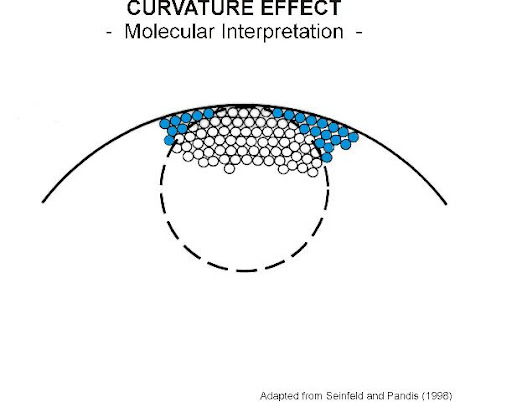
\includegraphics[trim=0 110 0 105, clip, width=\textwidth]
				{./images/Surface_t1}
%				\includegraphics[width=\textwidth]
%				{./images/Surface_t2}
%				물방울이 크기를 유지하기 위한 과포화도(supersaturation)
			\end{figure}
			물방울과 같이 표면이 휘어져 있으면 표면이 직선일 때보다 인접한 물 분자의 수가 줄어든다.\\
			이것으로 인해 물 분자에 작용하는 인력이 줄어들고, 증발이 쉽게 일어난다.\\

		\end{minipage}	
		&
		\begin{minipage}[t]{0.55\textwidth} \scriptsize

			\questionset{티끌이나 먼지를 함유하지 않은 매우 깨끗한 공기에서 상대습도가 100\%에 도달해도 물방울이 만들어지지 않는다. 왜 그럴까?}
			\solutionset{이러한 현상은 물방울의 표면 장력(surface tension)이 응결 작용을 방해하기 때문이다. 물방울이 형성될 때 수증기 분자가 들어가면 물방울의 표면적이 증가하므로 표면 장력을 고려해 볼 때, 수증기 분자가 물방울 속으로 들어가는 것은 어려운 상황이 된다. \newline}
			
			\questionset{구름 형성에 필요한 두 가지 중요한 요건은 무엇인가?}
			\solutionset{- 단열 냉각이나 수증기 공급에 의한 포화\\
				- 충분한 응결핵(응결에 필요한 표면) \newline}
			
			\questionset{구름 응결핵의 주된 공급원은 무엇인가?}
			\solutionset{먼지 폭풍, 화산 폭발, 식물의 꽃가루, 상물, 자동차, 석탄 연소 부산물, 해염 등}
		\end{minipage}
	\end{tabular}
\end{frame}



\begin{frame}[t]{퀼러 곡선}
	\begin{tabular}{ll}
		\begin{minipage}[t]{0.45\textwidth}\scriptsize
			\begin{figure}[t]
				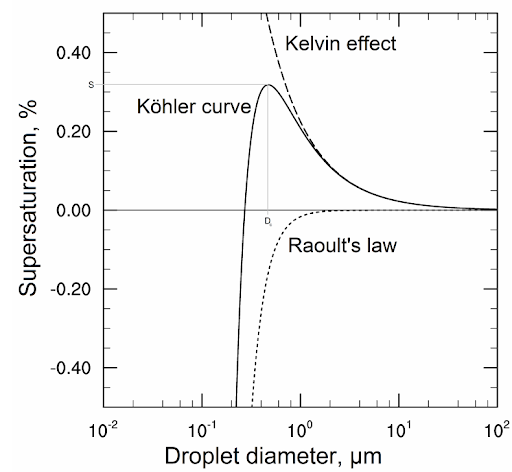
\includegraphics[trim=10 5 5 10, clip, width=\textwidth]
				{./images/Kohler_curve}
			\end{figure}
			
			
		\end{minipage}	
		&
		\begin{minipage}[t]{0.5\textwidth} \scriptsize
			\begin{itemize}
				\item 곡률 효과만 고려할 때 (켈빈 방정식): 크기가 작은 물방울이 쉽게 증발하므로 작은 물방울이 큰 물방울로 성장하기 어렵다 (물방울의 성장 억제)
				\item 용질 효과만 고려할 때 (라울의 법칙): 응결핵에 의해 순수하지 않은 상태가 되면 포화 수증기압의 감소로 큰 물방울로 성장하기 쉬워짐 (물방울의 성장 촉진)
			\end{itemize}
			
			\questionset{흡습성이 좋거나, 용해성이 좋은 에어로솔은 어떻게 응결 현상을 돕는가?}
			\solutionset{흡습성 에어로솔(곡률 효과와 관련): 물방울 크기 증가, 곡률 반지름 증가, 증기압 감소, 포화 수증기압 감소\\
				용해성 에어로솔(용질 효과와 관련): 용액 농도 증가, 증기압 감소, 포화 수증기압 감소 }
		\end{minipage}
	\end{tabular}
\end{frame}
\end{frame}


\begin{frame}[t]{구름 방울의 성장}
	\begin{tabular}{ll}
		\begin{minipage}[t]{0.55\textwidth} \scriptsize
			\begin{figure}[t]
				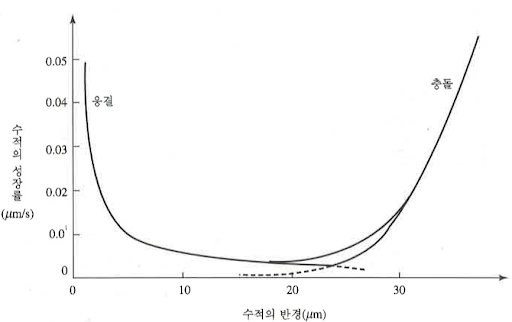
\includegraphics[width=\textwidth]{./images/colision}
			\end{figure}
		\end{minipage}	
		&
		\begin{minipage}[t]{0.4\textwidth} \scriptsize
			\begin{itemize}
				\item 초기에는 구름 방울이 응결 과정에 의해 빠르게 성장하나, 가용 수증기가 금새 소진되어 성장 속도가 느려짐.
				\item 물방울의 반경이 $20 \rm{~\mu m}$이하인 구름 방울이 형성됨.
				\item 큰 빗방울이 만들어지려면 구름 방울의 성장하는 과정이 필요함.
			\end{itemize}		
			
		\end{minipage}
	\end{tabular}
\end{frame}


\section{구름 분류}


\begin{frame}[t]{구름의 분류}
	\begin{tabular}{ll}
		\begin{minipage}[t]{0.90\textwidth}
			\begin{figure}[t]
				\includegraphics[trim=40 20 10 280, clip, page=156, width=0.8\textwidth]
				{\bookfile}
			\end{figure}
		\end{minipage}	
		&
		\begin{minipage}[t]{0.05\textwidth} \scriptsize
			
			
		\end{minipage}
	\end{tabular}
\end{frame}



\begin{frame}[t]{구름의 분류}
	\begin{tabular}{ll}
		\begin{minipage}[t]{0.3\textwidth}
			\begin{figure}[t]
				\includegraphics[trim=40 20 10 280, clip, page=156, width=\textwidth]
				{\bookfile}
			\end{figure}
		\end{minipage}	
		&
		\begin{minipage}[t]{0.65\textwidth} \scriptsize
			\begin{itemize}
			\item 영국의 박물학자 Luke Howard가 구름의 형태와 고도에 따라 분류
			\item 형태에 따라 \\
				권운(cirrus):높고 희며 얇다. 종종 깃털모양, \\
				적운(cumulus): 둥글고 개개의 구름 덩어리로 구성, \\
				층운(stratus): 홑이불 또는 층을 이루는 구름 \\
				난운(nimbus): 강수를 생산하는 구름의 이름을 뜻함 \\
			\item 모든 구름은 세 가지 기본 형태 중 하나를 반드시 가지며, 2가지의 결합체인 경우도 존재. 예를 들어 ‘층적운’, ‘권적운’, ‘권층운’과 같은 것. 
			\item 고도에 따라 \\
				상층운($6\rm{~km}$ 이상), 중층운($2\sim6\rm{~km}$), 하층운($2\rm{~km}$ 이하)으로 분류\\
			\item 연직 발달운(clouds of vertical development)은 하나의 고도 범위를 벗어나 연직으로 확장된 구름
			\item 해당 고도는 계절이나 위도에 따라 변할 수 있는데, 예를 들어 고위도의 겨울에는 상층운이 더 낮은 고도에 나타난다.
			\end{itemize}		
		\end{minipage}
	\end{tabular}
\end{frame}



\begin{frame}[t]{구름의 종류}
	\begin{tabular}{ll}
		\begin{minipage}[t]{0.90\textwidth}
				\begin{figure}[t]
					\includegraphics[trim=40 35 70 440, clip, page=157, width=0.9\textwidth]
					{\bookfile}
				\end{figure}
			\end{minipage}	
			&
			\begin{minipage}[t]{0.05\textwidth} \scriptsize
				
			\end{minipage}
			
		\end{tabular}
	\end{frame}
	




\begin{frame}[t]{상층운}
	낮은 기온과 적은 양의 수증기 때문에 엷고 희며, 얼음 결정으로 구성
	\begin{tabular}{ll}
		\begin{minipage}[t]{0.475\textwidth} \scriptsize
			\begin{figure}[t]
				\includegraphics[trim=20 500 335 50, clip, page=158, width=\textwidth]
				{\bookfile}
			\end{figure}
		권운: 가는 실 같은 얼음으로 구성된 구름
		\end{minipage}	
		&
		\begin{minipage}[t]{0.475\textwidth} \scriptsize
			\begin{figure}[t]
				\includegraphics[trim=350 500 10 50, clip, page=158, width=\textwidth]
				{\bookfile}
			\end{figure}
		권적운: 작은 공 모양의 덩어리가 뭉치거나 떨어지거나 하는 형태. 물고기 비늘과 유사			
		\end{minipage}

	\end{tabular}
\end{frame}


\begin{frame}[t]{상층운}
	낮은 기온과 적은 양의 수증기 때문에 엷고 희며, 얼음 결정으로 구성
	\begin{tabular}{ll}
		\begin{minipage}[t]{0.475\textwidth}\scriptsize
				\begin{figure}[t]
				\includegraphics[trim=20 230 335 295, clip, page=158, width=\textwidth]{\bookfile}
				\end{figure}
			권층운: 햇무리 달무리 만들때 잘 나타남. 때로는 너무 엷고 투명하여 식별하기 어려움.
			\end{minipage}	
			&
			\begin{minipage}[t]{0.475\textwidth} \scriptsize
				
				
			\end{minipage}

		\end{tabular}
\end{frame}



\begin{frame}[t]{중층운}
		\begin{figure}[t]
			\includegraphics[trim=20 410 30 50, clip, page=159, width=0.8\textwidth]{\bookfile}
		\end{figure}
	\begin{tabular}{ll}
		\begin{minipage}[t]{0.475\textwidth}\scriptsize
			고적운: 둥근 덩어리나 두루마리 형태의 큰 조각으로 형성. 보통 물방울로 이루어져 구름의 윤곽이 뚜렷함.
		\end{minipage}	
		&
		\begin{minipage}[t]{0.475\textwidth} \scriptsize
			고층운: 하늘의 많은 부분을 덮는 무정형의 회색 구름층. 이슬비 형태 강수 동반하기도 함.			
			
		\end{minipage}
		
	\end{tabular}
\end{frame}




\begin{frame}[t]{하층운}
	\begin{tabular}{ll}
		\begin{minipage}[t]{0.475\textwidth}\scriptsize
			\begin{figure}[t]
				\includegraphics[trim=20 0 350 505, clip, page=159, width=0.9\textwidth]{\bookfile}
			\end{figure}
			층적운: 길고 평행한 두루마리 혹은 부서진 공 모양으로 고적운과 유사하나 덩어리가  더 크게 부서진 조각임. 
		\end{minipage}	
		&
		\begin{minipage}[t]{0.475\textwidth} \scriptsize
			\begin{figure}[t]
				\includegraphics[trim=40 450 320 10, clip, page=160, width=0.8\textwidth]{\bookfile}
			\end{figure}
			난층운: 지속적인 강수와 낮은 시정거리. 공기가 전선을 따라 강제 상승할 때 처럼 안정한 조건에서 형성. 

		\end{minipage}
		
	\end{tabular}
\end{frame}






\begin{frame}[t]{연직 발달운}
	\begin{tabular}{ll}
		\begin{minipage}[t]{0.475\textwidth}\scriptsize
			\begin{figure}[t]
				\includegraphics[trim=40 40 350 450, clip, page=160, width=0.75\textwidth]{\bookfile}
			\end{figure}
				적운: 둥근 지붕이나 탑으로 발달하는 독립적 인 덩어리. 맑은날 비균등 지표 가열로 인해 공기가 상승응결고도 위로 상승할 때 형성
		\end{minipage}	
		&
		\begin{minipage}[t]{0.475\textwidth} \scriptsize
			\begin{figure}[t]
				\includegraphics[trim=360 40 10 350, clip, page=160, width=0.65\textwidth]{\bookfile}
			\end{figure}
				적란운: 크고 짙으며 부풀어 오른 모양. 거대한 탑 형태로 확장. 가끔 번개, 우박, 토네이도를 동반한 강한 비를 내리게 함.
			
		\end{minipage}
		
	\end{tabular}
\end{frame}





\begin{frame}[t]{다양한 구름들}
	\begin{tabular}{ll}
		\begin{minipage}[t]{0.4\textwidth}\scriptsize
			\begin{figure}[t]
				\includegraphics[trim=20 320 350 85, clip, page=161, width=0.9\textwidth]{\bookfile}
			\end{figure}
		\end{minipage}	
		&
		\begin{minipage}[t]{0.55\textwidth} \scriptsize
			\questionset{렌즈운(Lenticular clouds)이 형성되는 원리를 설명하시오.}
			\solutionset{정식 명칭은 렌즈 고적운(altocumulus lenticular)이라고 불리는데 산악 지형에서 주로 발생한다. 습하고 안정한 공기가 산을 넘어가면, 정상파가 풍하측에 형성된다. \\
			파의 마루로 공기가 상승함에 따라 공기덩이는 단열 냉각되어, 이슬점에 도달하게 되면 수증기가 응결되어 렌즈운이 된다. \\
			습한 공기가 하강하게 되어 파의 골에 도달하면 구름 입자들은 증발하여 해당 지역은 구름이 사라진다.}

		\end{minipage}
		
	\end{tabular}
\end{frame}






%\begin{frame}[t]{다양한 구름들}
%	\begin{tabular}{ll}
%		\begin{minipage}[t]{0.4\textwidth}\scriptsize
%			\begin{figure}[t]
%				\includegraphics[trim=320 320 50 185, clip, page=161, width=\textwidth]{\bookfile}
%			\end{figure}
%		\end{minipage}	
%		&
%		\begin{minipage}[t]{0.55\textwidth} \scriptsize
%			\questionset{지형성 구름(orographic clouds)에 속하는 불리는 모자 구름(cap cloud)의 형성과정을 설명하시오.}
%			\solutionset{모자 구}
%			
%		\end{minipage}
%		
%	\end{tabular}
%\end{frame}






\section{안개의 유형}


\begin{frame}[t]{안개}
	\begin{tabular}{ll}
		\begin{minipage}[t]{0.6\textwidth}\scriptsize
			\begin{figure}[t]
				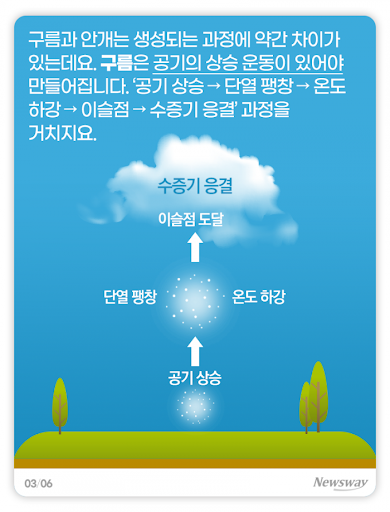
\includegraphics[width=0.48\textwidth]{./images/clouds.png} 	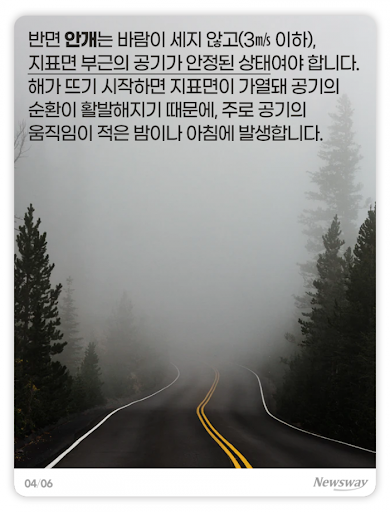
\includegraphics[width=0.48\textwidth]{./images/fog.png} 
			\end{figure}
		\end{minipage}	
		&
		\begin{minipage}[t]{0.35\textwidth} \scriptsize
			\questionset{구름과 안개의 차이점을 논하라.}
			\solutionset{중요한 차이점은 형성되는 장소와 방법이다. \\
				구름은 지표의 상공에서 형성되고 보통 상승하는 공기의 단열 냉각으로 형성된다. 반면 안개는 지표에서 형성되고 공기가 냉각되거나 수증기의 추가로 포화될 경우에 발생한다. \\
				안개는 본래 위험하지는 않지만 기상재해로 간주되며, 안개가 짙은 경우에는 시정을 크게 감소시켜서 위험한 상황을 만들 수 있다. }
		\end{minipage}
	\end{tabular}
\end{frame}




\begin{frame}[t]{안개의 종류}
	\begin{tabular}{ll}
		\begin{minipage}[t]{0.9\textwidth}\scriptsize
			\begin{figure}[t]
				\includegraphics[trim=30 520 50 50, clip, page=163, width=0.9\textwidth]{\bookfile}
			\end{figure}
		\end{minipage}	
		&
		\begin{minipage}[t]{0.05\textwidth} \scriptsize

		\end{minipage}
	\end{tabular}
		\begin{itemize}
			\item 냉각에 의해 형성되는 안개(fogs formed by cooling)
			\item 증발에 의해 형성되는 안개(fogs formed by the addition of water vapor)
		\end{itemize}	

\end{frame}





\begin{frame}[t]{복사 안개(radiation fog)}
	\begin{tabular}{ll}
		\begin{minipage}[t]{0.55\textwidth}\scriptsize
			
				\begin{figure}
				\begin{tikzpicture}
					\node[anchor=south west,inner sep=0] (image) at (0,0) {\includegraphics[trim=30 30 225 450, clip, page=162, width=\textwidth]{\bookfile}};
					\begin{scope}[x={(image.south east)},y={(image.north west)}]
						\filldraw[fill=white, draw = white] (0.5, 0.8) rectangle (1, 1);
						%\draw[help lines,xstep=.1,ystep=.1] (0,0) grid (1,1);
						%\foreach \x in {0,1,...,9} { \node [anchor=north] at (\x/10,0) {0.\x}; }
						%\foreach \y in {0,1,...,9} { \node [anchor=east] at (0,\y/10) {0.\y}; }
					\end{scope};
				\end{tikzpicture}
			\end{figure}

		\end{minipage}	
		&
		\begin{minipage}[t]{0.4\textwidth} \scriptsize
			\begin{itemize}
				\item 지표 및 지표 부근 공기의 복사 냉각으로 형성. 
				\item 맑고 상대습도가 높은 밤에 발생.
				\item 안개가 포함된 공기는 상대적으로 차갑고 밀도가 높아서 구릉성 지형에서 경사면을 따라 하강. 결국 골짜기에서 복사 안개가 가장 짙으며, 주변 산에서는 맑다. 
			\end{itemize}		
		\end{minipage}
	\end{tabular}
\end{frame}




\begin{frame}[t]{이류 안개(advection fog)}
	\begin{tabular}{ll}
		\begin{minipage}[t]{0.55\textwidth}\scriptsize
			
			\begin{figure}
				\begin{tikzpicture}
					\node[anchor=south west,inner sep=0] (image) at (0,0) {\includegraphics[trim=150 0 60 450, clip, page=163, width=\textwidth]{\bookfile}};
					\begin{scope}[x={(image.south east)},y={(image.north west)}]
						\filldraw[fill=white, draw = white] (0,1) rectangle (0.46, 0.8);
						%\draw[help lines,xstep=.1,ystep=.1] (0,0) grid (1,1);
						%\foreach \x in {0,1,...,9} { \node [anchor=north] at (\x/10,0) {0.\x}; }
						%\foreach \y in {0,1,...,9} { \node [anchor=east] at (0,\y/10) {0.\y}; }
					\end{scope};
				\end{tikzpicture}
			\end{figure}
		\end{minipage}	
		&
		\begin{minipage}[t]{0.4\textwidth} \scriptsize
			\begin{itemize}
				\item 고온 다습한 공기가 차가운 표면과 접촉하면 차가운 표면에 의해 생성된 차가운 공기와 섞이면서 대부분이 냉각되어 형성.
				\item ex) 금문교 근처의 이류 안개
			\end{itemize}		
		\end{minipage}
	\end{tabular}
\end{frame}




\begin{frame}[t]{활승 안개(upslope fog)}
	\begin{tabular}{ll}
		\begin{minipage}[t]{0.5\textwidth}\scriptsize
			\begin{figure}[t]
				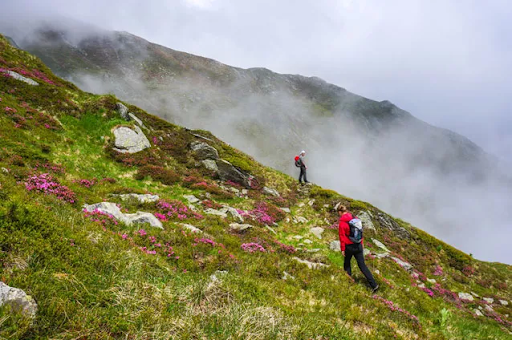
\includegraphics[width=\textwidth]{./images/upslope}
				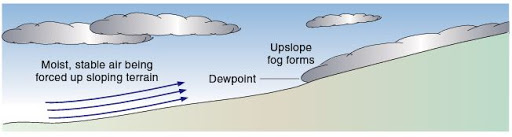
\includegraphics[width=\textwidth]{./images/upslope1} 
			\end{figure}
		\end{minipage}	
		&
		\begin{minipage}[t]{0.45\textwidth} \scriptsize
			\begin{itemize}
				\item 습윤한 공기가 완만하게 경사진 평원을 따라 이동하거나 가파른 산의 경사면을 따라 상승할 경우에 생성. 
				\item 상승에 의해 단열 팽창하면서 형성됨
			\end{itemize}		
		\end{minipage}
	\end{tabular}
\end{frame}




\begin{frame}[t]{김 안개(steam fog)}
	\begin{tabular}{ll}
		\begin{minipage}[t]{0.5\textwidth}\scriptsize
			\begin{figure}[t]
				\includegraphics[trim=0 430 320 0, clip, page=164, width=\textwidth]{\bookfile}
			\end{figure}
		\end{minipage}	
		&
		\begin{minipage}[t]{0.45\textwidth} \scriptsize
			\begin{itemize}
				\item 차가운 공기가 따뜻한 수면 위로 이동하면 충분한 양의 수분이 수면에서 증발하여 수면 바로 위의 공기를 포화시킴.
				\item 맑고 선선한 가을아침 호수와 강에서 많이 발생
				\item 증발 안개, 물 안개 라고도 함.				
			\end{itemize}		
		\end{minipage}
	\end{tabular}
\end{frame}




\begin{frame}[t]{전선 안개(frontal fog) 또는 강수 안개(precipitation fog)}
	\begin{tabular}{ll}
		\begin{minipage}[t]{0.45\textwidth} \scriptsize
			\begin{figure}[t]
				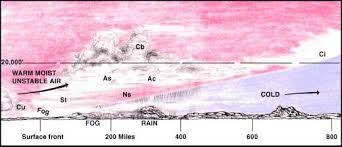
\includegraphics[width=\textwidth]{./images/frontal_fog}
			\end{figure}
		\end{minipage}	
		&
		\begin{minipage}[t]{0.5\textwidth} \scriptsize
			\begin{itemize}
				\item 따뜻한 공기가 차가운 공기 위로 이동하면서 비가 내리고 아래의 차가운 공기가 거의 포화상태에서 내린 비가 증발하여 안개를 형성할 수 있다. 
			\end{itemize}		
		\end{minipage}
	\end{tabular}
\end{frame}


\begin{frame}[t]{안개 발생}
	\begin{tabular}{ll}
		\begin{minipage}[t]{0.55\textwidth}\scriptsize
			\begin{figure}[t]
				\includegraphics[trim=40 0 240 500, clip, page=166, width=0.9\textwidth]{\bookfile}
			\end{figure}
		\end{minipage}	
		&
		\begin{minipage}[t]{0.4\textwidth} \scriptsize
			\questionset{태평양 연안에서 짙은 안개가 상대적으로 자주 발생하는 이유는 무엇인가?}
			\solutionset{태평양의 따뜻하고 습한 공기가 북아메리카의 서부 연안을 평행하게 따라 흐르는 차가운 해류에 의해 냉각되면서 이류 안개를 형성한다.\newline}

			\questionset{복사 안개가 상승한다고 할 때, 실제로 어떤 현상이 일어나는가?}
			\solutionset{복사 안개가 상승한다는 말을 사용하지만 실제로 안개가 상승하는 것은 아니다. 태양이 지면을 따뜻하게 하면, 지면 근처의 공기 덩이가 가열되고, 안개는 바닥에서부터 증발하게 되어 마치 안개가 상승한 것처럼 보인다. \newline }
		\end{minipage}
	\end{tabular}
\end{frame}




\begin{frame}[t]{안개 지도}
	\begin{tabular}{ll}
		\begin{minipage}[t]{0.75\textwidth}\scriptsize
			\begin{figure}[t]
				\includegraphics[trim=280 30 30 519, clip, page=164, width=\textwidth]{\bookfile}
			\end{figure}
		\end{minipage}	
		&
		\begin{minipage}[t]{0.2\textwidth} \scriptsize
				
		\end{minipage}
	\end{tabular}
\end{frame}








\section{강수는 어떻게 형성되는가}


\begin{frame}[t]{강수 형성}
	\begin{tabular}{ll}
		\begin{minipage}[t]{0.45\textwidth}\scriptsize
			\begin{figure}[t]
				\includegraphics[trim=30 30 360 510, clip, page=165, width=\textwidth]{\bookfile}
			\end{figure}
		\end{minipage}	
		&
		\begin{minipage}[t]{0.5\textwidth} \scriptsize
			\questionset{구름 입자와 빗방울의 지름은 100배 정도 차이가 난다. 이것이 의미하는 바는 무엇인가?}
			\solutionset{구름 입자가 모여 빗방울이 되려면 100 만 개 정도가 모여야 한다. 이는 증발하지 않고 지면에 도달하기에 충분한 빗방울을 만들기 위해서는 응결 외에 추가적인 과정이 필요함을 알려준다.}
				
		\end{minipage}
	\end{tabular}
\end{frame}




\begin{frame}[t]{빙정설(베르예론 과정, Bergeron)}
	\begin{tabular}{ll}
		\begin{minipage}[t]{0.5\textwidth}\scriptsize
			\begin{figure}[t]
				\includegraphics[trim=50 430 330 50, clip, page=166, width=0.9\textwidth]{\bookfile}
			\end{figure}
		\end{minipage}	
		&
		\begin{minipage}[t]{0.45\textwidth} \scriptsize
			한랭 구름(cold cloud)에는 \\
					$-40 \rm{{^\circ}C}$ 미만: 완전히 얼음 결정 \\
					$-40 \rm{{^\circ}C} \sim -15 \rm{{^\circ}C}$: 과냉각 물방울, 얼음 공존 \\
					$-15 \rm{{^\circ}C} \sim 0 \rm{{^\circ}C}$: 대부분 과냉각 물방울\\
			
			\begin{itemize}
				\item 과냉각 수: 공기 중의 순수한 물은 -40℃에 이르기 전에 얼지 않음. $0 \rm{{^\circ}C}$ 아래의 액체 상태의 물을 과냉각수라고 부름
				\item 결빙핵: 과냉각 물방울과 접촉하여 얼게 만드는 고체 입자로 얼음 결정과 비슷한 모양을 가진다. 대기 중 희박하게 존재 \\
			\end{itemize}		
		
		\end{minipage}
	\end{tabular}
\end{frame}






\begin{frame}[t]{빙정설(베르예론 과정, Bergeron)}
	\begin{tabular}{ll}
		\begin{minipage}[t]{0.4\textwidth}\scriptsize
			\begin{figure}[t]
				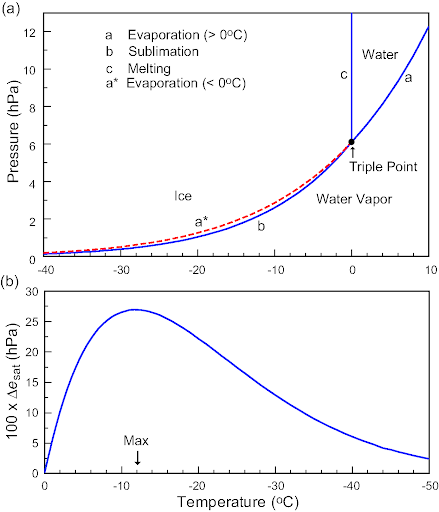
\includegraphics[width=\textwidth]{./images/e}
			\end{figure}
		\end{minipage}	
		&
		\begin{minipage}[t]{0.55\textwidth} \scriptsize
			\begin{figure}[t]
				\includegraphics[trim=355 360 40 260, clip, page=166, width=0.7\textwidth]{\bookfile}
			\end{figure}
			\begin{itemize}
				\item 얼음 결정이 액체 물방울보다 결속이 더 강하기 때문에 각 면에서 출입하는 물분자의 수는 얼음이 과냉각수보다 적음.
				\item 과냉각 물방울보다 얼음 결정 위에서 포화수증기압이 더 낮음. ($-12 \rm{{^\circ}C}$ 부근에서 차이가 가장 큼)
			\end{itemize}		
			
		\end{minipage}
	\end{tabular}
\end{frame}



\begin{frame}[t]{빙정설(베르예론 과정, Bergeron)}
	\begin{tabular}{ll}
		\begin{minipage}[t]{0.4\textwidth}\scriptsize
			\begin{figure}[t]
				\includegraphics[trim=45 310 340 50, clip, page=167, width=0.8\textwidth]{\bookfile}
			\end{figure}
		\end{minipage}	
		&
		\begin{minipage}[t]{0.55\textwidth} \scriptsize
			\begin{itemize}
				\item 과냉각 물방울과 빙정의 포화수증기압 차이로 인해 물방울 근처 수증기가 빙정 근처로 이동. 
				\item 과냉각 물방울의 수증기압을 낮추므로 물방울면에서는 불포화, 빙정면에서는 과포화 상태.
				\item 이에 따라 물방울에서 증발한 수증기가 빙정에 승화하여 빙정이 성장하게 됨. (침적(deposition))
				\item 침적에 의해 어느 정도 크기가 커지면 빙정 또는 과냉각 물방울과 충돌하여 빨리 성장함 (부착(aggregation))
				\item 즉, 빙정이 충분히 커지면 중력에 의해 지표 방향으로 낙하. 
				\item 부숴지면 새로운 결빙핵이 되어 연쇄 반응에 의해 많은 눈결정이 형성되며, 이러한 눈결정이 뭉쳐져서 눈송이와 같은 더 큰 덩어리가 됨.

			\end{itemize}		
			
		\end{minipage}
	\end{tabular}
\end{frame}





\begin{frame}[t]{종단 속도}
	\begin{tabular}{ll}
		\begin{minipage}[t]{0.45\textwidth} \scriptsize
			\begin{figure}[t]
				\includegraphics[trim=330 55 40 590, clip, page=167, width=\textwidth]{\bookfile}
			\end{figure}
		\end{minipage}	
		&
		\begin{minipage}[t]{0.5\textwidth} \scriptsize
			\begin{itemize}
				\item 비가 내리기 위해서는 충돌 과정 또는 병합 과정을 통한 성장이 필요
				\item 물방울의 반경이 $20 \rm{~\mu m}$보다 큰 구름 방울이 있어야 충돌 과정 또는 병합 과정에 의해 빗방울 형성 가능.
				\item 종단 속도는 물체가 낙하할 때 최대 속도이며, 공기 저항과 중력의 크기가 같을 때 생기는 속도임. 
				\item 큰 물방울의 종단 속도가 작은 물방울의 종단 속도보다 크기 때문에 더 빨리 떨어지므로 충돌 및 병합이 발생함. 
			\end{itemize}		

		\end{minipage}
	\end{tabular}
\end{frame}






\begin{frame}[t]{충돌 병합}
	\begin{tabular}{ll}
		\begin{minipage}[t]{0.60\textwidth}\scriptsize
			\begin{figure}[t]
				\includegraphics[trim=90 465 370 60, clip, page=168, width=0.48\textwidth]{\bookfile} 		\includegraphics[trim=90 200 370 340, clip, page=168, width=0.48\textwidth]{\bookfile}
			\end{figure}
		\end{minipage}	
		&
		\begin{minipage}[t]{0.35\textwidth} \scriptsize
			\begin{itemize}
				\item 온난 구름은 구름 꼭대기의 온도가 $-15 \rm{{^\circ}C} \sim 0 \rm{{^\circ}C}$ 보다 높아 빙정이 없다.
				\item 큰 구름 방울들이 낙하 속도가 빨라 작은 구름 방울을 낚아채 커진다.
				\item 커진 구름 방울은 낙하 속도가 증가하고 그 결과 공기 저항도 증가하여 빗방울이 편평해 진다.				
				\item 빗방울이 $4 \rm{~mm} $에 이르면 바닥에 저압부가 발달한다.
				\item 빗방울이 지름 $5 \rm{~mm} $를 초과하면 저기압이 폭발적으로 위로 성장해서 금새 작은 물방울로 부서지는 도넛 모양의 물의 링을 형성한다. 
				
			\end{itemize}		
			
		\end{minipage}
	\end{tabular}
\end{frame}


\begin{frame}[t]{충돌 병합}
	\begin{tabular}{ll}
		\begin{minipage}[t]{0.65\textwidth}\scriptsize
			\questionset{충돌-병합 과정이 Bergeron 과정과 다른 점은 무엇인가?}
			\solutionset{Bergeron 과정은 온도가 영하인 차가운 구름에서 일어난다. 그리고 응결핵과는 달리 빙정핵은 매우 드물어서 빙정 성장에 일부 도움만 줄 뿐이다. 반면에 충돌-병합 과정은 영상의 따뜻한 구름에서 일어나 강수를 형성한다. \\
			충돌-병합 과정에서는 큰 물방울의 낙하 속도가 상대적으로 빨라 작은 물방울을 휩쓸고 지나가면서 성장하게 되고 5mm 정도로 커진 물방울은 다시 조각나 낙하 속도가 차이 나는 또 다른 물방울 성장 동력으로 작용하게 된다. \newline}
		
			\questionset{중위도에서는 충돌-병합과정이 Bergeron 과정과 협력하여 대형 적란운에 의한 강수를 설명할 수 있다. 어떤 과정으로 강수를 설명하는가?}
			\solutionset{적란운 상부에서 베르예론 과정은 눈을 생성하는데, 결빙고도 아래를 지나면서 녹는다. 눈송이들은 녹으면서 낙하속도가 빠른 비교적 큰 물방울들을 형성한다. 이 큰 물방울들이 하강해서 구름의 하부 영역 대부분을 차지하고 있는 느리고 작은 구름방울을 따라 잡아 병합한다. 그 결과 폭우가 내릴 수 있다. }

		\end{minipage}	
		&
		\begin{minipage}[t]{0.3\textwidth} \scriptsize
			\begin{figure}[t]
				
			\end{figure}
			
		\end{minipage}
	\end{tabular}
\end{frame}








\section{강수의 형태}


\begin{frame}[t]{비, 눈}
		
		\begin{figure}[t]
			\includegraphics[trim=45 255 50 330, clip, page=169, width=\textwidth]
			{\bookfile}
		\end{figure}
		
	\begin{tabular}{ll}
		\begin{minipage}[t]{0.475\textwidth} \scriptsize
			비: 상층은 영하지만, 하강할수록 온도가 상승하여 지표면 근처 상공부터 지표면까지 온도가 영상인 경우에 해당\\
			이슬비: 지름이 $0.5\rm{~mm}$ 미만인 빗방울\\
			박무(mist): 지면에 닿을 수 있는 매우 작은 물방울을 포함한 강수(안개와 유사)\\
		\end{minipage}	
		&
		\begin{minipage}[t]{0.475\textwidth} \scriptsize
			눈: 눈은 얼음 결정 집합체 형태의 겨울 강수의 한 종류\\
			싸락눈(graupel): 낙하하는 눈 결정들이 과냉각 구름방울을 포획하여 성장한 결과(결착) 고유의 육면체 눈 결정 모양을 알아볼 수 없는 경우\\
		\end{minipage}
		
	\end{tabular}
\end{frame}


\begin{frame}[t]{꼬리 구름}
	\begin{tabular}{ll}
		\begin{minipage}[t]{0.5\textwidth}\scriptsize
			\begin{figure}[t]
				\includegraphics[trim=250 0 0 480, clip, page=170, width=0.9\textwidth]{\bookfile}
			\end{figure}
			
		\end{minipage}	
		&
		\begin{minipage}[t]{0.45\textwidth} \scriptsize
			\questionset{꼬리 구름은 무엇이며 어떤 조건에서 형성되는가?}
			\solutionset{비가 구름 아래에 있는 불포화 공기와 만나게 되면 증발하기 시작하는데, 공기의 수분과 물방울의 크기에 따라 비가 지면에 닿기 전에 완전히 증발되는 경우 꼬리 구름이 형성될 수 있다.}
			
		\end{minipage}
	\end{tabular}
\end{frame}


\begin{frame}[t]{진눈개비, 언 비}
	\begin{figure}[t]
		\includegraphics[trim=45 35 50 540, clip, page=169, width=\textwidth]
		{\bookfile}
	\end{figure}
	\begin{tabular}{ll}
		\begin{minipage}[t]{0.475\textwidth} \scriptsize
			진눈개비(sleet): 눈이 낙하하면서 영상인 기층을 통과하여 녹았다가, 지표에 도달하기 전에 다시 영하층을 통과하여 얼게 되면서 얼음싸라기로 지면에 도달하는 것
		\end{minipage}	
		&
		\begin{minipage}[t]{0.475\textwidth} \scriptsize	
			언 비(freezing rain) 또는 비얼음(glaze): 눈이 낙하하면서 영상인 기층을 통과하여 녹았다가, 지표면에 도달하기 전에 다시 영하층을 통과하여 과냉각 물방울로 지면에 도달하여 지면의 물체와 접촉하는 순간 얼음으로 변화하는 것
		\end{minipage}
		
	\end{tabular}
\end{frame}



\begin{frame}[t]{강수 형태}
	\begin{tabular}{ll}
		\begin{minipage}[t]{0.9\textwidth} \scriptsize
			\begin{figure}[t]
				\includegraphics[trim=50 400 40 50, clip, page=170, width=0.9\textwidth]
				{\bookfile}
			\end{figure}
		\end{minipage}	
		&
		\begin{minipage}[t]{0.05\textwidth} \scriptsize	

		\end{minipage}
		
	\end{tabular}
\end{frame}





\begin{frame}[t]{진눈개비와 언비의 형성}
	\begin{tabular}{ll}
		\begin{minipage}[t]{0.65\textwidth}\scriptsize
			\begin{figure}[t]
				\includegraphics[trim=50 300 30 50, clip, page=172, width=\textwidth]{\bookfile}
			\end{figure}
			
		\end{minipage}	
		&
		\begin{minipage}[t]{0.3\textwidth} \scriptsize
			\begin{itemize}
				\item 눈이 낙하하면서 겪는 주위 기온이 영하일 경우 지상에서 눈으로 내릴 수 있으나,
				\item 낙하하면서 겪는 기온과 해당 경로의 길이에 따라 지상에서 강수의 형태는 달라진다. 
					
			\end{itemize}		

		\end{minipage}
	\end{tabular}
\end{frame}


\begin{frame}[t]{진눈개비와 비얼음}
\begin{tabular}{ll}
	\begin{minipage}[t]{0.4\textwidth}\scriptsize
		\begin{figure}[t]
			\includegraphics[trim=50 270 350 50, clip, page=173, width=0.7\textwidth]{\bookfile}
		\end{figure}
		
	\end{minipage}	
	&
	\begin{minipage}[t]{0.55\textwidth} \scriptsize
		\questionset{진눈깨비와 비얼음이 무엇인지 설명하라. 두 형태의 강수가 형성되는 조건은 어떻게 다른가?}
		\solutionset{진눈깨비는 눈이 낙하하면서 따듯한 기층을 통과하여 녹았다가 지표에 도달하기 전에 다시 차가운 층을 통과하게 되어 얼게 되면서 얼음싸라기로 지면에 도달하는 것을 말하며, \\
		비얼음은 눈이 낙하도중 따뜻한 기층을 통과하여 녹았다가 다시 차가운 기층을 통과해 오면서 다시 과냉각물방울로 지면에 도달하게 되어 지면의 물체와 접촉하는 순간 다시 얼음으로 변화하는 것을 말함.\\}
		
	\end{minipage}
\end{tabular}
\end{frame}




%비는 지름이 최소 0.5mm 이상인 물방울로 제한
%대부분의 비는 난층운 또는 적란운에서 생성되나 지름이 0.5mm 미만인 물방울은 이슬비로 불리며 보통 층운이나 난층운에서 생성
%박무는 지면에 닿을 수 있는 매우 작은 물방울을 포함한 강수를 뜻함
%
%
%
%
%눈은 얼음결정 집합체 형태의 겨울 강수의 한 종류
%매우 낮은 온도에서 공기의 수분함량이 작을 때 형성된 매우 가벼운 눈을 가루눈이라 하며, -5℃보다 따뜻한 기온의 얼음 결정은 서로 엉겨서 더 큰 덩어리가 되어 무겁고 수분이 많은 눈이 된다.
%낙하하는 눈결정이 미세한 과냉각 구름방울을 포획하면서 성장하여 고유의 육면체 눈결정 모양을 알아볼 수 없게 되면, 이러한 눈을 싸락눈이라고 한다.
%
%상층에서 지표면까지 계속 영하일 때 해당












\begin{frame}[t]{눈 결정}
	\begin{tabular}{ll}
		\begin{minipage}[t]{0.42\textwidth}\scriptsize
			\begin{figure}[t]
				\includegraphics[trim=50 50 290 490, clip, page=171, width=0.9\textwidth]{\bookfile}
			\end{figure}
			
		\end{minipage}	
		&
		\begin{minipage}[t]{0.53\textwidth} \scriptsize
				\questionset{눈 결정 모양이 육각형 구조를 하는 이유는 무엇인가?}
				\solutionset{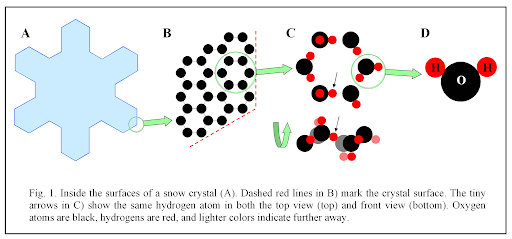
\includegraphics[width=0.9\textwidth]{./images/66}\\
					물 분자의 결합각이 $104.5\rm{^\circ}$이며, 얼음의 경우 육각형 모양의 안정한 수소 결합을 함에 따라 눈 결정의 모양이 육각형의 구조를 갖게 된다. \newline}
				
				\questionset{눈 결정 모양에 영향을 미치는 요인은 무엇인가?}
				\solutionset{먼저 온도에 따라 눈 결정이 판형, 기둥형 등의 모양을 갖게 되며, 여기에  수증기에 대한 과포화 정도에 따라 눈 결정의 모양이 달라지게 된다.}
			
		\end{minipage}
	\end{tabular}
\end{frame}




\begin{frame}[t]{우박}
	\begin{tabular}{ll}
		\begin{minipage}[t]{0.4\textwidth}\scriptsize
			\begin{figure}[t]
				\includegraphics[trim=325 320 50 40, clip, page=173, width=0.9\textwidth]{\bookfile}
			\end{figure}
			
		\end{minipage}	
		&
		\begin{minipage}[t]{0.55\textwidth} \scriptsize	
				\questionset{우박은 어떻게 형성되고 어떤 요소가 우박의 최종 크기를 결정하는가?}
				\solutionset{우박은 상승기류가 충분히 강하고, 과냉각 물방울이 충분한 적란운에서 생성된다.\\
				작은 얼음 핵이 구름 사이를 통과하면서 떨어질 때 과냉각 물방울을 수집하여 성장하게 되고, 강한 상승기류를 만나 다시 위로 올라가면서 과냉각 물방울을 수집하여 성장하고 다시 떨어지면서 성장하기를 반복한다.\\ 이러한 과정을 반복할수록 우박의 크기는 성장하게 되는데, 우박의 최종 크기를 결정하는 것은 결국 상승기류의 강도, 과냉각 물방울의 양, 구름을 통과한 경로의 길이라 할 수 있다.\\
				그러다 하강기류를 만나거나 너무 무거워지면 지표로 떨어는데, 농작물이 상하거나 시설물 파괴 등의 피해를 발생시킨다.}
		\end{minipage}
	\end{tabular}
\end{frame}



\begin{frame}[t]{상고대}
	\begin{tabular}{ll}
		\begin{minipage}[t]{0.4\textwidth}\scriptsize
			\begin{figure}[t]
				\includegraphics[trim=350 350 50 50, clip, page=174, width=0.9\textwidth]{\bookfile}
			\end{figure}
			
		\end{minipage}	
		&
		\begin{minipage}[t]{0.55\textwidth} \scriptsize	
			\questionset{상고대는 무엇이며, 어떤 경우에 형성되는가?}
			\solutionset{상고대는 과냉각된 안개 또는 구름 방울들이 물에체 접촉하여 얼어 붙을때 형성된다.}
			
		\end{minipage}
	\end{tabular}
\end{frame}












\section{강수 측정}




\begin{frame}[t]{우량계}
	\begin{tabular}{ll}
		\begin{minipage}[t]{0.60\textwidth}\scriptsize
			\begin{figure}[t]
				\includegraphics[trim=45 50 80 480, clip, page=177, width=\textwidth]{\bookfile}
			\end{figure}
			
		\end{minipage}	
		&
		\begin{minipage}[t]{0.35\textwidth} \scriptsize	
			\questionset{뚜껑이 없는 통이 우량계를 대신할 수 있지만 표준 우량계를 더 많이 쓴다. 표준 우량계를 사용할 때의 이점은 무엇인가?}
			\solutionset{표준 우량계는 빗물이 들어오면 원통 모양의 측정 튜브로 안내한다. 그런데 튜브의 단면적이 빗물 수신부의 약 $\frac{1}{10}$ 크기이기 때문에 실제 강우량을 $10$ 배 만큼 확대시킬 수 있어 높은 정확도로 측정할 수 있다. \\
				또한 상부의 지름이 약 $20 \rm{~cm}$로 작아서 이러한 형태가 증발을 억제시켜 정확한 측정이 가능하도록 돕는다.}
			
		\end{minipage}
	\end{tabular}
\end{frame}



\begin{frame}[t]{우량계}
	\begin{tabular}{ll}
		\begin{minipage}[t]{0.475\textwidth}\scriptsize
			\questionset{표준 우량계 외에 사용하는 강수 측정 도구는 무엇인지 설명하시오.}
			\solutionset{전도형 우량계는 일정한 양만큼(보통 $0.02\rm{~cm}$)의 빗물이 수집되면 물통이 기울어져서 물을 비워내는데, 물통이 기울어질 때마다 전기회로가 차단되어 이러한 변화가 기록장치에 연속적으로 기록된다. 저울 우량계는 강수를 저울 위의 원통에 모은 뒤, 원통이 다 차면 움직임이 데이터를 기록하는 펜으로 전달한다. 	}
			
		\end{minipage}	
		&
		\begin{minipage}[t]{0.475\textwidth} \scriptsize	
			\questionset{강수량의 측정을 부정확하게 하는 요소는 무엇인가?}
			\solutionset{전도식 우량계는 물통이 기울어지는 동안 빗물을 모을 수 없어 약 25\% 과소 측정\\
				바람의 존재는 강수가 너무 많이 혹은 너무 적게 들어가게 하여 오차 유발\\
				측정 지역의 위치에 따른 노출 환경이 측정의 오차 유발	}
			
		\end{minipage}
	\end{tabular}
\end{frame}



\begin{frame}[t]{전지구 강수 관측 (Global Precipitation Measurement)}
	\begin{tabular}{ll}
		\begin{minipage}[t]{0.5\textwidth}\scriptsize
			\begin{figure}[t]
				\includegraphics[trim=200 260 40 150, clip, page=178, width=\textwidth]{\bookfile}
			\end{figure}

		\end{minipage}	
		&
		\begin{minipage}[t]{0.45\textwidth} \scriptsize	
			\begin{itemize}
				\item Tropical Rainfall Measuring Mission (TRMM) : 열대지역과 아열대지역의 강수를 측정하기 위해 1997년에 그 임무를 시작
				\item Global Precipitation Measurement(GPM) : 
				인공위성 자료를 이용하는 강수량 추정에는 일반적으로 적외선, 마이크로파가 사용된다.\\
				적외선 방법은 구름층을 통과할 수 없기 때문에 운정 온도, 구름의 면적, 형태 등의 여러 특성을 이용하는 간접적인 강수 추정방법 (정지 위성, 시간적인 분해능이 탁월)\\
				마이크로파 방법은 마이크로파가 강수층을 통과할 때 강수 입자에 의해 산란되거나, 또는 강수층에서 방출되는 성질을 이용하는 직접적인 강수 추정 방법(극궤도 위성, 하루에 2회 정도의 관측)
				
			\end{itemize}
			
		\end{minipage}
	\end{tabular}
\end{frame}




\begin{frame}[t]{기상 레이다(Doppler radar)}
	\begin{tabular}{ll}
		\begin{minipage}[t]{0.45\textwidth}\scriptsize
			\begin{figure}[t]
				\includegraphics[trim=25 330 270 50, clip, page=179, width=0.9\textwidth]{\bookfile}
			\end{figure}

		\end{minipage}	
		&
		\begin{minipage}[t]{0.5\textwidth} \scriptsize	
			기상 레이다는 발신기로 짧은 펄스 신호를 송출한 후 반사되는 신호를 이용하여 물체를 감지한다. 강수를 감지하기 위해서 $3\sim10\rm{~nm}$의 파장이 이용된다.\\
			
			\questionset{기상 레이다의 장점과 단점은 무엇인가?}
			\solutionset{장점은 표준 우량계이 비해 넓은 범위의 강수를 실시간으로 관측할 수 있다는 것이고,\\
			단점은 곤충떼를 구별하지 못하고, 고체 형태의 강수를 구별하지 못한다.}
			
		\end{minipage}
	\end{tabular}
\end{frame}



\begin{frame}[t]{기상 레이다(weather radar)}
	\begin{tabular}{ll}
		\begin{minipage}[t]{0.45\textwidth}\scriptsize
			\begin{figure}[t]
				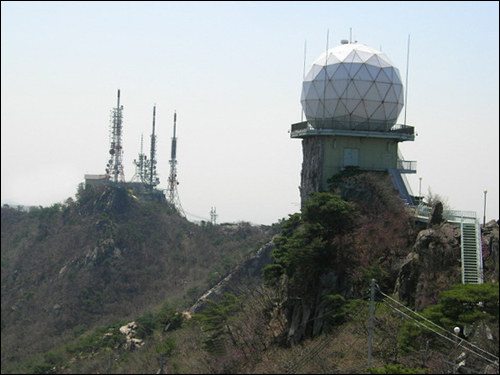
\includegraphics[width=\textwidth]{./images/radar2}
			\end{figure}
			
		\end{minipage}	
		&
		\begin{minipage}[t]{0.5\textwidth} \scriptsize	
			
			\questionset{우리나라에 기상 레이더는 몇 기가 설치되어 있는가?}
			\solutionset{성산, 구덕산, 면봉산, 관악산, 백령도, 오성산, 진도, 광덕산, 강릉, 고산 (10곳), 인천공항 추가\\
				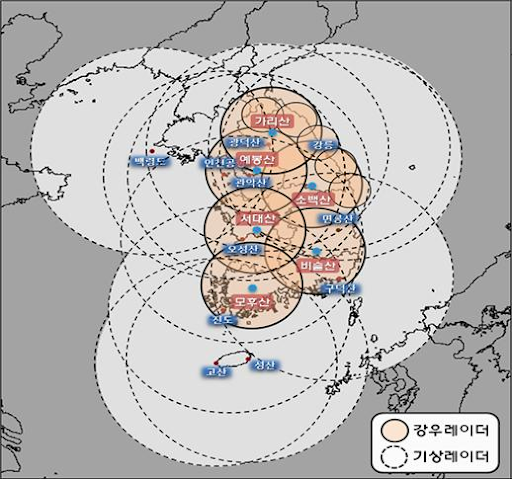
\includegraphics[width=0.8\textwidth]{./images/radar1}}
			
		\end{minipage}
	\end{tabular}
\end{frame}


\section{계획적 및 비의도적 기상조절}


\begin{frame}[t]{구름 씨뿌리기}
	\begin{tabular}{ll}
		\begin{minipage}[t]{0.4\textwidth}\scriptsize
			\begin{figure}[t]
				\includegraphics[trim=50 320 320 50, clip, page=180, width=0.9\textwidth]{\bookfile}
			\end{figure}

		\end{minipage}	
		&
		\begin{minipage}[t]{0.55\textwidth} \scriptsize	
			\questionset{구름 씨뿌리기가 성공하기 위해서는 특정 기상 조건이 만족되어야 한다. 그 기상 조건은 무엇인가?}
			\solutionset{일단 구름이 있어야 하고, 구름의 일부는 과냉각되어 있어야 한다. \newline}
			
			\questionset{과냉각 구름에 대한 씨뿌리기에 아이오딘화 은 결정이 사용되는 이유는?}
			\solutionset{아이오딘화 은 결정은 얼음과 유사한 구조를 가지고 있어 과냉각 물방울로부터 수증기가 달라붙게 하여 빙정을 형성하게 함으로써 Bergeron 과정을 촉진시킬 수 있다.}
			
		\end{minipage}
	\end{tabular}
\end{frame}



\begin{frame}[t]{우박 억제}
	\begin{tabular}{ll}
		\begin{minipage}[t]{0.4\textwidth}\scriptsize
			\begin{figure}[t]
				\includegraphics[trim=350 40 20 350, clip, page=180, width=0.9\textwidth]{\bookfile}
			\end{figure}

		\end{minipage}	
		&
		\begin{minipage}[t]{0.55\textwidth} \scriptsize	
			\questionset{우박 억제에 대한 현대적 시도는 무엇인가?}
			\solutionset{우박 덩이의 성장을 중단시키기 위해 요오드화 은 결정을 이용하는 다양한 구름 씨뿌리기 방법을 행해 왔으나. 씨를 뿌린 구름과 뿌리지 않은 구름들 사이에서 우발 박생에 대해 통계적으로 유의한 차이가 없음이 밝혀졌다.}
			
		\end{minipage}
	\end{tabular}
\end{frame}




\begin{frame}[t]{서리 방지}
	\begin{tabular}{ll}
		\begin{minipage}[t]{0.6\textwidth}\scriptsize
			\begin{figure}
			\begin{tikzpicture}
				\node[anchor=south west,inner sep=0] (image) at (0,0) {\includegraphics[trim=40 350 80 50, clip, page=181, width=0.9\textwidth]{\bookfile}};
				\begin{scope}[x={(image.south east)},y={(image.north west)}]
					\filldraw[fill=white, draw = white] (0.5, 0.25) rectangle (1, 0);
					%\draw[help lines,xstep=.1,ystep=.1] (0,0) grid (1,1);
					%\foreach \x in {0,1,...,9} { \node [anchor=north] at (\x/10,0) {0.\x}; }
					%\foreach \y in {0,1,...,9} { \node [anchor=east] at (0,\y/10) {0.\y}; }
				\end{scope};
			\end{tikzpicture}
		\end{figure}
	
		\end{minipage}	
		&
		\begin{minipage}[t]{0.35\textwidth} \scriptsize	
			\questionset{과수원 난로(orchard heater), 스프링 클러 및 공기 혼합이 서리 방지에 어떻게 이용되는지 서술하라.}
			\solutionset{Orchard heater는 기온이 영상이 되도록 연료를 이용하여 충분한 열을 만들어 내는 역할을 하고, \\
			스프링 클러는 물을 분사하여 물 자체가 가지고 있는 온도(기온보다 물이 고온이라는 가정하에)와 물이 얼면서 방출하는 잠열을 이용하여 영하로 
			떨어지는 것을 막는 역할을 하고, \\
			공기 혼합은 차가운 지면의 공기와 상대적으로 따뜻한 상공의 공기를 섞어서 지면의 기온을 높이는 역할을 한다. }
			
		\end{minipage}
	\end{tabular}
\end{frame}



\begin{frame}[t]{비행운}
	\begin{tabular}{ll}
		\begin{minipage}[t]{0.45\textwidth}\scriptsize
			\begin{figure}[t]
				\includegraphics[trim=350 440 30 50, clip, page=182, width=0.9\textwidth]{\bookfile}
			\end{figure}
		\end{minipage}	
		&
		\begin{minipage}[t]{0.5\textwidth} \scriptsize	
			\questionset{비행운은 어떠한 경우 형성되며 비행운이 기후에 미치는 영향은 무엇인가? }
			\solutionset{비행운은 항공기의 엔진에서 나오는 황산염이 응결핵 역할을 하고 배기가스의 수증기가 해당 공기를 포화시키면서 발생한다. \\
				주로 $–50\rm{^\circ}$ 이하의 고도($9\rm{~km}$)에서 형성된다. 9.11 테러시 3일간 민간 항공기의 비행이 금지되었는데 일교차가 $1.1\rm{^\circ}$ 증가하였다. 이로부터 비행운이 입사 태양 복사 에너지를 줄이고, 지구 복사에너지도 줄이는 효과를 가지고 있는 것으로 나타났다. }
			
		\end{minipage}
	\end{tabular}
\end{frame}


\begin{frame}[t]{도시 효과}
	\begin{tabular}{ll}
		\begin{minipage}[t]{0.4\textwidth}\scriptsize
%			\begin{figure}[t]
%				\includegraphics[trim=350 420 50 50, clip, page=182, width=0.9\textwidth]{\bookfile}
%			\end{figure}
		\end{minipage}	
		&
		\begin{minipage}[t]{0.55\textwidth} \scriptsize	
			\questionset{도시 및 도시의 풍하 쪽에서 많은 강수를 생성하는 데 기여하는 세 가지 요소는 무엇인가? }
			\solutionset{도시의 온도가 높아 공기의 상승으로 인해 단열 냉각이 일어나 구름이 생길 가능성이 높으며,\\
				공해물질과 먼지 등의 요인으로 인해서 응결핵이 많으며, \\
				풍하 측에서 기온이 급감하면서 상대습도가 급격히 높아질 가능성이 크기 때문이다.}
			
		\end{minipage}
	\end{tabular}
\end{frame}



